\documentclass[11pt,a4paper]{article}

\usepackage[margin=2.5cm]{geometry}
\usepackage[T1]{fontenc}
\usepackage[utf8]{inputenc}
\usepackage{lmodern}
\usepackage{microtype}
\usepackage{graphicx}
\usepackage{booktabs}
\usepackage{array}
\usepackage{longtable}
\usepackage{enumitem}
\usepackage{hyperref}
\usepackage{float}
\usepackage{amsmath}
\usepackage{caption}

\hypersetup{
    colorlinks=true,
    linkcolor=black,
    urlcolor=blue,
    citecolor=black
}

\captionsetup{font=small}
\renewcommand{\arraystretch}{1.15}

% Adjust this if needed
\newcommand{\dbms}{PostgreSQL}

\title{Phase 1 Report\\Conceptual and Logical Design of the \texttt{APP\_SNAPSHOT} Data Mart}
\author{}
\date{}

\begin{document}
\maketitle

\section{Introduction}
This report presents the Phase 1 design of the data mart built for the Google Play Store project. The design follows the data-driven methodology studied during the course. Starting from the reconciled relational schema, we identify the fact of interest, build and edit the attribute tree, define dimensions and measures, derive the final Dimensional Fact Model (DFM) schema, and finally translate the conceptual schema into a logical relational schema for ROLAP analysis.

The final result of Phase 1 is a data mart centered on the fact \texttt{APP\_SNAPSHOT}, modeled conceptually through a DFM schema and implemented logically as a star schema extended with a bridge table for the multiple arc involving \texttt{Genre}.

\section{Data Source and Preliminary Requirement Analysis}

\subsection{Data Source}
The project is based on a Google Play Store dataset containing information about mobile applications published in the store. The data includes both descriptive information about applications and quantitative attributes observed at snapshot level, such as rating, number of reviews, number of installs, price, size, and last update date.

From an analytical point of view, this source is appropriate for multidimensional design because it provides:
\begin{itemize}[leftmargin=1.5em]
    \item descriptive attributes that can be organized into dimensions, such as app, category, app type, content rating, and genre;
    \item numerical attributes that can be analyzed as measures;
    \item a temporal business attribute (\texttt{last\_updated\_date}) supporting time-based analysis;
    \item a non-trivial structural aspect, namely the many-to-many association between snapshots and genres.
\end{itemize}

\subsection{Preliminary Requirement Analysis}
The goal of the data mart is to support exploratory and aggregate analysis of the observed state of applications in the store. In particular, the design is intended to support questions such as:
\begin{itemize}[leftmargin=1.5em]
    \item how ratings, reviews, and installs vary across categories;
    \item how free and paid apps differ in price and popularity;
    \item how content rating is associated with the main numerical indicators;
    \item how application snapshots can be analyzed over time through the update date;
    \item how genre-based analyses can be performed despite the many-to-many relationship with app snapshots.
\end{itemize}

These requirements motivate the choice of a snapshot-oriented fact and a star schema suitable for OLAP-style aggregation and slicing.

\section{Reconciled Source Schema and Data-Driven Design Approach}

\subsection{Re-engineering Step}
The original source data was first reorganized into a reconciled relational schema. This re-engineering step makes the source more suitable for subsequent data warehouse design by separating descriptive entities, identifying relationships explicitly, and preparing the data for the data-driven conceptual modeling process.

The reconciled database was implemented in \dbms. This report starts from that reconciled layer and derives the conceptual and logical schemas of the data mart.

\subsection{Schema of the Reconciled Database}
Figure~\ref{fig:reconciled_schema} shows the reconciled relational schema used as input for the data-driven design. The central relation is \texttt{reconciled.app\_snapshot}, which stores the snapshot-level numerical attributes and business descriptors. The descriptive tables \texttt{reconciled.app}, \texttt{reconciled.category}, \texttt{reconciled.app\_type}, and \texttt{reconciled.content\_rating} provide the main candidates for dimensions. Moreover, the association \texttt{reconciled.app\_snapshot\_genre} captures the many-to-many relationship between snapshots and genres, which later motivates the multiple arc in the DFM schema and the bridge table in the logical design.

\begin{figure}[H]
    \centering
    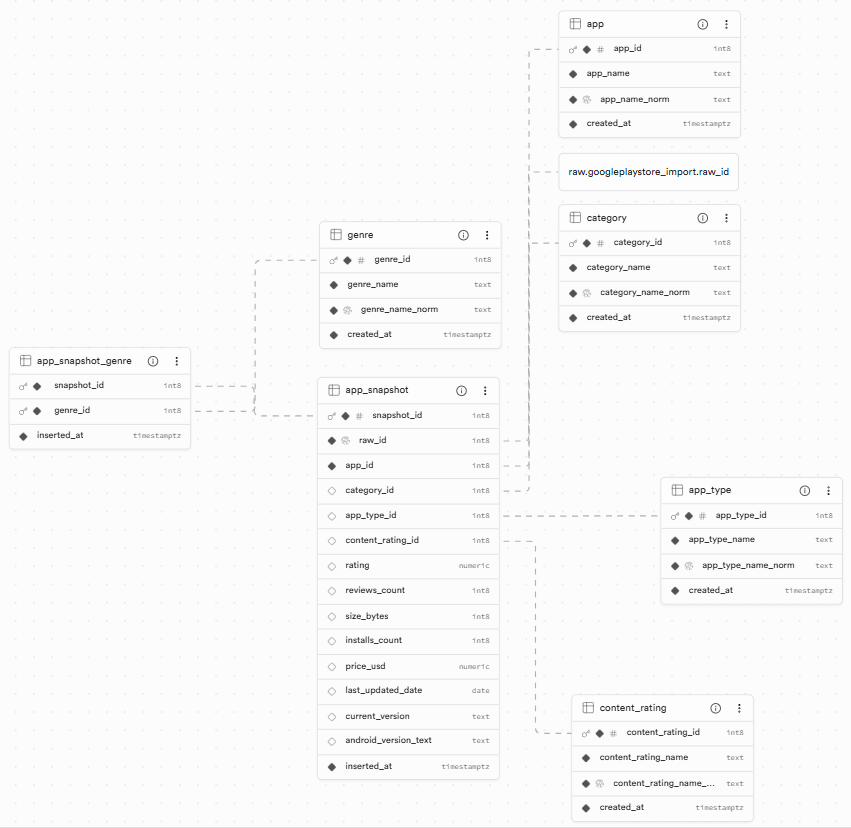
\includegraphics[width=\textwidth]{./figures/reconciledSchema.png}
    \caption{Reconciled relational schema used as input for the data-driven design.}
    \label{fig:reconciled_schema}
\end{figure}

The reconciled schema is implemented in \dbms\ and represents the starting point for the data-driven workflow.

\subsection{data-driven Design Workflow}
The design follows the data-driven workflow adopted in class:
\begin{enumerate}[leftmargin=1.5em]
    \item definition of the fact;
    \item construction of the basic attribute tree;
    \item editing of the attribute tree;
    \item definition of dimensions;
    \item definition of measures;
    \item design of the final fact schema;
    \item translation into a logical star schema.
\end{enumerate}

\section{Conceptual Design}

\subsection{Definition of the Fact}
The fact chosen for the analysis is \texttt{APP\_SNAPSHOT}. This choice is motivated by the nature of the relation: it represents a dynamic phenomenon of interest for decision-making, namely the observed state of an application at a specific observation point. Each record contains quantitative properties such as rating, number of reviews, number of installs, price, and size, which make the relation suitable for multidimensional analysis.

In contrast, tables such as \texttt{app}, \texttt{category}, \texttt{app\_type}, and \texttt{content\_rating} contain mostly descriptive and relatively stable data, and are therefore more appropriate as dimensions.

At conceptual level, the grain of the fact can be described as one observed snapshot of one application at one update date.

\subsection{Construction of the Basic Attribute Tree}
Starting from the reconciled schema, the basic attribute tree is built by taking the identifier of \texttt{APP\_SNAPSHOT} as the root and recursively following attributes and to-one associations. The resulting tree includes:
\begin{itemize}[leftmargin=1.5em]
    \item direct numerical attributes of \texttt{app\_snapshot}: \texttt{rating}, \texttt{reviews\_count}, \texttt{installs\_count}, \texttt{price\_usd}, \texttt{size\_bytes};
    \item business attributes such as \texttt{last\_updated\_date}, \texttt{current\_version}, and \texttt{android\_version\_text};
    \item to-one related descriptive entities: \texttt{app}, \texttt{category}, \texttt{app\_type}, and \texttt{content\_rating}.
\end{itemize}

The relation \texttt{app\_snapshot\_genre} is not part of the basic attribute tree because it represents a to-many association. Therefore, it does not belong to the basic recursive construction based only on functional dependencies and to-one associations.

\begin{figure}[H]
    \centering
    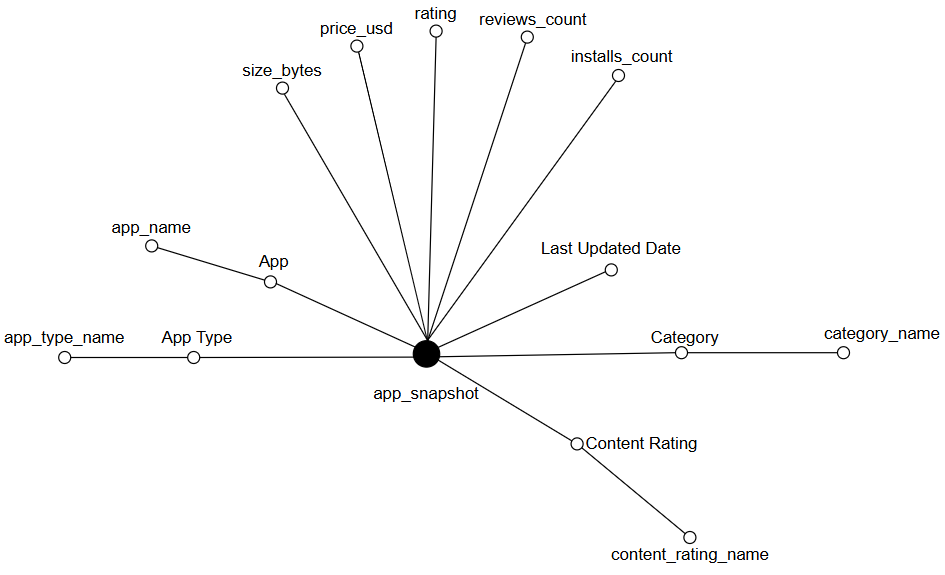
\includegraphics[width=0.9\textwidth]{./figures/attributeTree.png}
    \caption{Basic attribute tree of \texttt{APP\_SNAPSHOT}. The tree includes the direct numerical attributes, the business date \texttt{last\_updated\_date}, and the descriptive entities reachable through to-one associations. The to-many association with \texttt{Genre} is intentionally excluded at this stage.}
    \label{fig:basic_tree}
\end{figure}

\subsection{Editing of the Attribute Tree}
The attribute tree is then edited through pruning and grafting operations.

\paragraph{Pruned elements.}
The following technical attributes are removed because they are not useful for aggregation at the conceptual level:
\begin{itemize}[leftmargin=1.5em]
    \item \texttt{snapshot\_id} in the conceptual representation;
    \item \texttt{raw\_id};
    \item the technical identifiers \texttt{app\_id}, \texttt{category\_id}, \texttt{app\_type\_id}, and \texttt{content\_rating\_id} as labels of intermediate nodes.
\end{itemize}

In addition, \texttt{current\_version} and \texttt{android\_version\_text} are pruned from the conceptual schema because they are not used to define aggregation paths in the current analysis scenario.

\paragraph{Grafted elements.}
The technical identifiers of related tables are replaced by business dimensions and their descriptive leaves:
\begin{itemize}[leftmargin=1.5em]
    \item \texttt{App} $\rightarrow$ \texttt{app\_name}
    \item \texttt{Category} $\rightarrow$ \texttt{category\_name}
    \item \texttt{App Type} $\rightarrow$ \texttt{app\_type\_name}
    \item \texttt{Content Rating} $\rightarrow$ \texttt{content\_rating\_name}
\end{itemize}

\paragraph{Time dimension.}
The business attribute \texttt{last\_updated\_date} is transformed into the temporal dimension \texttt{Date}, with hierarchy:
\[
\texttt{Date} \rightarrow \texttt{day} \rightarrow \texttt{month} \rightarrow \texttt{year}
\]
This hierarchy is used as the temporal dimension of the fact schema.

\paragraph{Advanced construct.}
The association with \texttt{Genre} is reintroduced at the conceptual level as a multiple arc. This modeling choice is required because the reconciled schema shows that the same app snapshot may be associated with more than one genre.

\subsection{Definition of Dimensions}
After editing the attribute tree, the selected dimensions are:
\begin{itemize}[leftmargin=1.5em]
    \item \texttt{App}
    \item \texttt{Category}
    \item \texttt{App Type}
    \item \texttt{Content Rating}
    \item \texttt{Date}
\end{itemize}

These dimensions determine the granularity of the primary events represented by the fact. The \texttt{Genre} dimension is modeled separately through a multiple arc because its relationship with the fact is many-to-many.

\subsection{Definition of Measures}
The measures are the numerical attributes directly associated with each snapshot:
\begin{itemize}[leftmargin=1.5em]
    \item \texttt{rating}
    \item \texttt{reviews\_count}
    \item \texttt{installs\_count}
    \item \texttt{price\_usd}
    \item \texttt{size\_bytes}
\end{itemize}

From the point of view of additivity, \texttt{rating}, \texttt{price\_usd}, and \texttt{size\_bytes} are treated as non-additive measures. The measures \texttt{reviews\_count} and \texttt{installs\_count} are snapshot-based measures and therefore must be handled carefully along the temporal hierarchy, since summing them across time for the same app may lead to double counting of successive observations.

\subsection{Final DFM Schema}
The final conceptual schema is centered on the fact \texttt{APP\_SNAPSHOT}. The dimensions and hierarchies are:
\begin{itemize}[leftmargin=1.5em]
    \item \texttt{App} $\rightarrow$ \texttt{app\_name}
    \item \texttt{Category} $\rightarrow$ \texttt{category\_name}
    \item \texttt{App Type} $\rightarrow$ \texttt{app\_type\_name}
    \item \texttt{Content Rating} $\rightarrow$ \texttt{content\_rating\_name}
    \item \texttt{Date} $\rightarrow$ \texttt{day} $\rightarrow$ \texttt{month} $\rightarrow$ \texttt{year}
\end{itemize}

The measures are \texttt{rating}, \texttt{reviews\_count}, \texttt{installs\_count}, \texttt{price\_usd}, and \texttt{size\_bytes}.

The final DFM schema also includes an advanced construct: \texttt{Genre} is represented as a \emph{multiple arc}. This modeling choice is required because the reconciled schema contains the relation \texttt{app\_snapshot\_genre}, and data inspection confirmed that the same snapshot may be associated with more than one genre.

\begin{figure}[H]
    \centering
    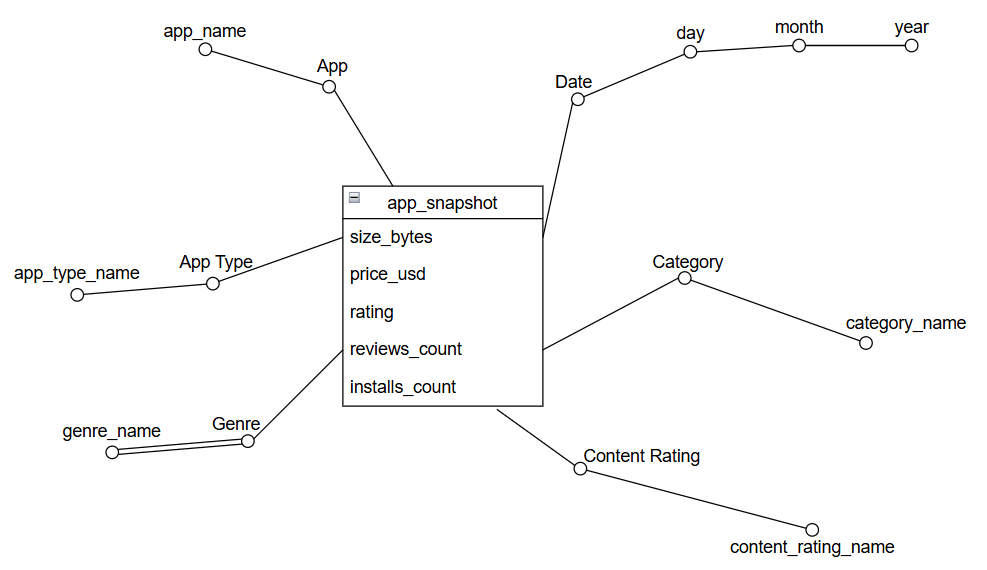
\includegraphics[width=0.92\textwidth]{./figures/DFM_Schema.png}
    \caption{Final DFM schema for \texttt{APP\_SNAPSHOT}. The figure shows the fact, the selected dimensions and hierarchies, and the multiple arc with \texttt{Genre}.}
    \label{fig:dfm_schema}
\end{figure}

\section{Logical Design}

\subsection{Choice of the Logical Model}
The conceptual schema is translated into a ROLAP logical model. The chosen implementation is a star schema. Since the conceptual schema contains a multiple arc involving \texttt{Genre}, the final logical solution is a star schema extended with a bridge table.

The logical schema is also designed for implementation in \dbms.

\subsection{Dimension Tables}
The following dimension tables are created:
\begin{itemize}[leftmargin=1.5em]
    \item \texttt{dim\_app(app\_key, app\_id, app\_name)}
    \item \texttt{dim\_category(category\_key, category\_id, category\_name)}
    \item \texttt{dim\_app\_type(app\_type\_key, app\_type\_id, app\_type\_name)}
    \item \texttt{dim\_content\_rating(content\_rating\_key, content\_rating\_id, content\_rating\_name)}
    \item \texttt{dim\_last\_updated\_date(last\_updated\_date\_key, full\_date, day, month, year)}
    \item \texttt{dim\_genre(genre\_key, genre\_id, genre\_name)}
\end{itemize}

Each dimension table is identified by a surrogate key and stores the business key coming from the reconciled schema. At logical level, the conceptual dimension \texttt{Date} is implemented through the table \texttt{dim\_last\_updated\_date}, in order to preserve traceability to the source attribute \texttt{last\_updated\_date}.

\subsection{Fact Table}
The fact table is:
\begin{quote}
\texttt{fact\_app\_snapshot(app\_snapshot\_key, snapshot\_id, app\_key, category\_key, app\_type\_key,} \\
\texttt{content\_rating\_key, last\_updated\_date\_key, rating, reviews\_count, installs\_count,} \\
\texttt{price\_usd, size\_bytes)}
\end{quote}

The grain of the fact table is one row for each row of \texttt{reconciled.app\_snapshot}. The attribute \texttt{snapshot\_id} is retained as a business key to preserve traceability with the reconciled layer, while \texttt{app\_snapshot\_key} is the surrogate primary key of the fact table.

\subsection{Bridge Table for the Multiple Arc}

The many-to-many relationship between app snapshots and genres is implemented through the bridge table shown in Figure~\ref{fig:logical_schema}:
\begin{quote}
\texttt{bridge\_app\_snapshot\_genre(app\_snapshot\_key, genre\_key, weight)}
\end{quote}

The primary key of the bridge table is the pair \texttt{(app\_snapshot\_key, genre\_key)}. The attribute \texttt{weight} is used to support weighted analyses over the multiple arc. In the implemented loading workflow, the weight is computed as:
\[
\texttt{weight} = \frac{1}{\texttt{number of genres associated with the snapshot}}
\]

Data checks confirmed that:
\begin{itemize}[leftmargin=1.5em]
    \item the minimum weight is \texttt{0.5};
    \item the maximum weight is \texttt{1.0};
    \item the sum of the weights for each \texttt{app\_snapshot\_key} is equal to \texttt{1}.
\end{itemize}

\subsection{Handling Missing Dimension Values}
During the loading phase, one source row was found to contain missing values for both \texttt{content\_rating\_id} and \texttt{last\_updated\_date}. To avoid excluding this row from the fact table, two special members are introduced at the logical level:
\begin{itemize}[leftmargin=1.5em]
    \item an \texttt{Unknown} member in \texttt{dim\_content\_rating};
    \item an \texttt{Unknown Date} member in \texttt{dim\_last\_updated\_date}, represented by \texttt{1900-01-01}.
\end{itemize}

This choice does not change the conceptual design. It only affects the logical loading strategy and makes the data mart robust to incomplete source records.

\subsection{Indexes and Constraints}
The implemented logical schema includes:
\begin{itemize}[leftmargin=1.5em]
    \item primary keys on all dimension tables and on the fact table;
    \item a unique constraint on \texttt{fact\_app\_snapshot.snapshot\_id};
    \item foreign key constraints from the fact table to the dimensions;
    \item a primary key on \texttt{bridge\_app\_snapshot\_genre(app\_snapshot\_key, genre\_key)};
    \item a \texttt{NOT NULL} and \texttt{CHECK} constraint on the bridge attribute \texttt{weight};
    \item indexes on the main foreign keys to improve join performance.
\end{itemize}

\subsection{Glossary of the Measures}
Table~\ref{tab:measure_glossary} provides a glossary of the measures used in the data mart.

\begin{longtable}{@{}p{2.8cm}p{5.2cm}p{2.0cm}p{4.8cm}@{}}
\caption{Glossary of the measures.}
\label{tab:measure_glossary}\\
\toprule
\textbf{Measure} & \textbf{Meaning} & \textbf{Unit} & \textbf{Aggregation behavior} \\
\midrule
\endfirsthead

\toprule
\textbf{Measure} & \textbf{Meaning} & \textbf{Unit} & \textbf{Aggregation behavior} \\
\midrule
\endhead

\bottomrule
\endfoot

\texttt{rating} & Observed average user rating of the app at snapshot time. & score & Non-additive. Typically analyzed through averages rather than sums. \\

\texttt{reviews\_count} & Number of user reviews observed for the app at snapshot time. & count & Snapshot-based. It can be aggregated across non-temporal dimensions, but summing it across time for the same app may double count successive observations. \\

\texttt{installs\_count} & Number of installs observed for the app at snapshot time. & count & Snapshot-based. It can be aggregated across non-temporal dimensions, but summing it across time for the same app may double count successive observations. \\

\texttt{price\_usd} & Observed app price at snapshot time. & USD & Non-additive. Typically analyzed through averages, minima, maxima, or distributions. \\

\texttt{size\_bytes} & Observed app size at snapshot time. & bytes & Non-additive. Typically analyzed through averages, minima, maxima, or distributions. \\
\end{longtable}

\begin{figure}[H]
    \centering
    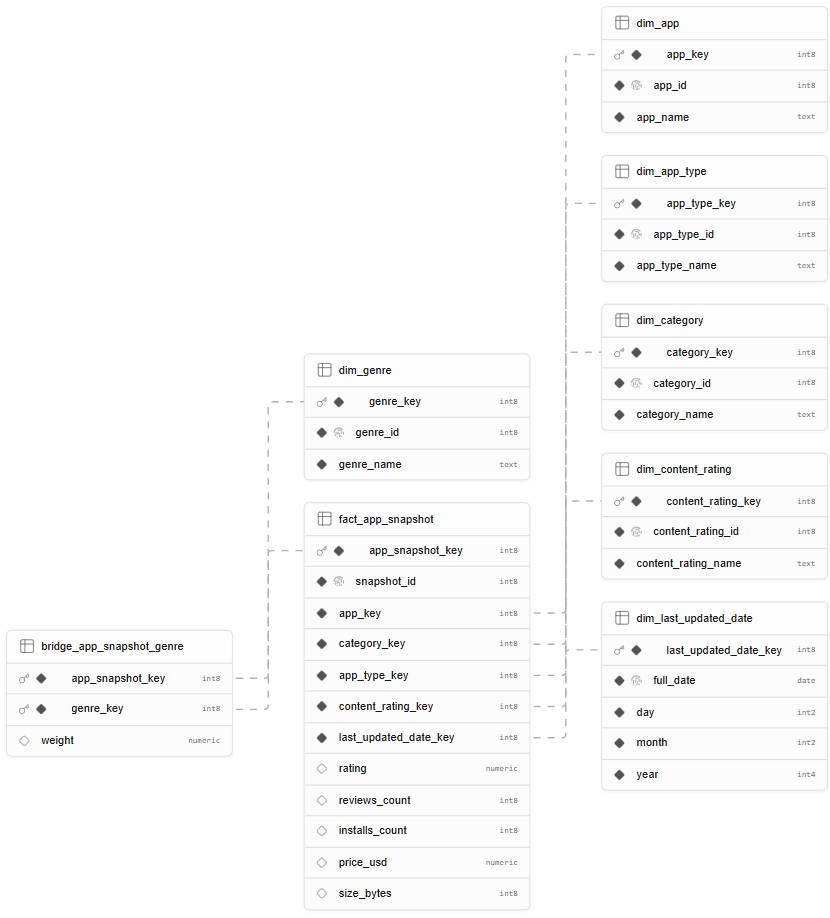
\includegraphics[width=0.9\textwidth]{./figures/starSchema.png}
    \caption{Logical star schema for \texttt{APP\_SNAPSHOT}, extended with a bridge table for \texttt{Genre}.}
    \label{fig:logical_schema}
\end{figure}

\section{Brief Note on Data Quality and Cleaning Tasks}
A preliminary inspection of the reconciled data already revealed some quality issues relevant to the design:
\begin{itemize}[leftmargin=1.5em]
    \item one source row contains missing values for \texttt{content\_rating\_id} and \texttt{last\_updated\_date};
    \item the relationship between app snapshots and genres is many-to-many and therefore requires explicit handling in the conceptual and logical schemas;
    \item snapshot-based numerical attributes such as \texttt{reviews\_count} and \texttt{installs\_count} require careful interpretation along the temporal hierarchy.
\end{itemize}

These observations influenced the Phase 1 design, especially the introduction of Unknown members in the logical schema, the bridge table for \texttt{Genre}, and the interpretation of snapshot-based measures. A more detailed treatment of data quality assessment and cleaning tasks belongs to the following project phase.

\section{Final Result of Phase 1}
Phase 1 produces the following outputs:
\begin{enumerate}[leftmargin=1.5em]
    \item the identification of \texttt{APP\_SNAPSHOT} as the fact of interest;
    \item the construction and editing of the attribute tree;
    \item the final DFM schema with dimensions, measures, and the multiple arc for \texttt{Genre};
    \item the logical translation into a star schema with a bridge table;
    \item a consistent loading strategy that preserves all source records by mapping missing dimension values to Unknown members.
\end{enumerate}

\section{Conclusion}
The Phase 1 design of the data mart is complete. The conceptual design is consistent with the data-driven methodology studied during the course, and the logical design correctly translates the DFM schema into a relational structure suitable for OLAP analysis. The final solution can be described as a star schema for \texttt{APP\_SNAPSHOT}, extended with a bridge table to implement the multiple arc with \texttt{Genre}. This design preserves the multidimensional semantics of the phenomenon of interest while providing a practical and robust implementation for the data mart.

\end{document}